\documentclass[12pt, a4paper]{article}
\usepackage[outputdir=out]{minted}
\usepackage[utf8]{inputenc}
\usepackage{geometry}
\usepackage[italian]{babel}
\usepackage{graphicx}
\usepackage[belowskip=-15pt,aboveskip=0pt]{caption}
\usepackage{enumitem}

\setlist{nosep}

\graphicspath{{images/}}

\geometry {   
    top=20mm,
    bmargin=20mm
}
\begin{document}

\begin{titlepage}
    \centering

    \vspace{0.5cm} {
        \large Politecnico di Milano\\
    }

    \vspace{5cm} {
        \huge {
            Progetto di Reti Logiche 2021/2022\\
        }
        \vspace{0.5cm}
        \large {Scaglione Prof. Salice}
    }

    \vspace{2cm} {
        \large
        Edoardo Fullin ( Codice Persona 10677606)
    }

    \vspace*{\fill}
    \today

\end{titlepage}

\tableofcontents

\pagebreak

\section{Introduzione}

\subsection{Descrizione del progetto}

Lo scopo del progetto è il design, tramite linguaggio VHDL di un modulo hardware sintetizzabile per FPGA
in grado di applicare ad una sequenza di parole in input un codice convoluzionale $1/2$, che 
può essere implementato attraverso la macchina a stati finiti in figura.


\begin{figure}[!ht]
    \centering
    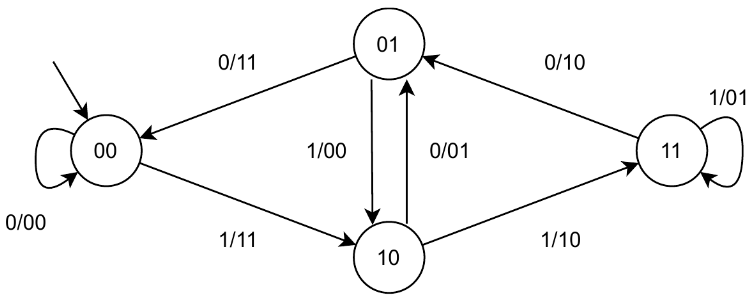
\includegraphics[scale=0.7]{convoluzionatore_1_2_fsm.png}
    \caption{FSM convoluzionatore $1/2$}
    \label{fig:fsm_conv}
\end{figure}

Il modulo deve quindi restituire in output (scrivendo in memoria) le uscite della macchina a stati finiti,
bit per bit. % dire meglio

\subsection{Esempio}

La FSM prende in input la parola \verb+11001011+, che deve essere serializzata come
1 al tempo 0, 1 al tempo 1, 0 al tempo 2 e così via.
La macchina quindi, partendo dallo stato di reset 00 andrà nello stato 10 alla lettura
del primo 1 producendo in output 11, passerà poi nello stato 3 producendo 10, nello stato 01
producendo 10 e nello stato 00 producendo 11.
Il primo byte di output sarà quindi 11100111, che dovrà essere scritto in memoria.
Si nota quindi facilmente che la lunghezza della sequenza di output è esattamente doppia di quella 
dell'input.

\pagebreak

\subsection{Specifiche del modulo da realizzare}

Il modulo da descrivere è sincrono sincronizzato su un clock 'globale', non include la memoria su cui viene effettuato input/output e
deve implementare la seguente interfaccia verso l'esterno:

\begin{minted}[]{vhdl}
    
    entity project_reti_logiche is
        port (
            i_clk : in std_logic;
            i_rst : in std_logic;
            i_start : in std_logic;
            i_data : in std_logic_vector(7 downto 0);
            o_address : out std_logic_vector(15 downto 0);
            o_done : out std_logic;
            o_en : out std_logic;
            o_we : out std_logic;
            o_data : out std_logic_vector (7 downto 0)
        );
    end project_reti_logiche;

\end{minted}

In particolare:

\begin{itemize}
    \item \texttt{i\_clk} è il segnale di clock, generato dall'esterno
    \item \texttt{i\_rst} è il segnale di reset
    \item \texttt{i\_start} è il segnale di inizio sequenza
    \item \texttt{i\_data} è il byte in arrivo dalla memoria RAM
    \item \texttt{o\_address} è l'indizzo di memoria da cui si vuole leggere/scrivere
    \item \texttt{o\_done} è il segnale di fine computazione
    \item \texttt{o\_en} è il segnale di enable per la memoria RAM
    \item \texttt{o\_we} è il segnale di scrittura per la memoria RAM
    \item \texttt{o\_data} è il byte da scrivere in memoria RAM
\end{itemize}

\pagebreak

\section{Architettura}

La architettura del componente è composta principalmente da due moduli: una macchina a stati di controllo
e da un datapath che gestisce il flusso dati.
La FSM di controllo ha il compito di generare i segnali di controllo che attivano, disattivano o modificano
il comportamento dei sottomoduli del datapath in base allo stato attuale della esecuzione.
Il datapath gestisce l'intero flusso di dati, dalla lettura della memoria di input alla serializzazione, 
alla bufferizzazione del risultato e alla sua scrittura in memoria.

\noindent Vengono illustrati più in dettaglio i singoli componenti.

\subsection{Datapath}

Il datapath è il componente che si occupa della gestione del flusso dati, incluso l'input e l'output
da e verso la memoria RAM.
Nella attuale implementazione è stata usata una solo entity VHDL, che può essere vista come l'insieme
di più moduli collegati tra loro come dallo schema in figura.
I componenti del datapath sono pilotati dai segnali di controllo generati dalla macchina a stati che
controlla il flusso di esecuzione.

\begin{figure}[h!]
    \centering
    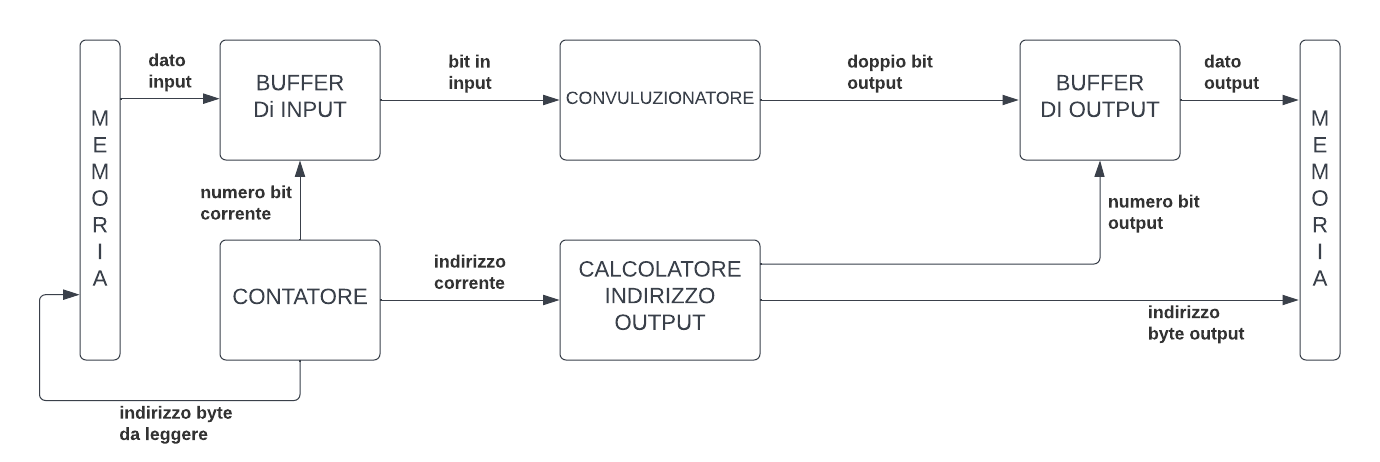
\includegraphics[scale=0.32]{datapath.png}
    \label{fig:datapath_small}
    \caption{Schema ad alto livello del componente datapath, schema più dettagliato a pagina XXX} %% TODO
\end{figure}

\subsubsection{Input Buffer}

Il buffer di input è realizzato con un registro (entity \texttt{serializer\_register}) che, in presenza del segnale 
\texttt{sr\_byte\_load} memorizza il dato attualmente presente sul bus \texttt{i\_data} e lo tiene memorizzato.
Il registro ha un parametro aggiuntivo \texttt{i\_sel} di lunghezza 3 bit (0-7)
che permette di specificare quale singolo bit interno al byte memorizzato si vuole in ouput.

\subsubsection{Contatore}

Il contatore è un semplice contatore da 11 bit che tiene traccia del numero del bit corrente,
in questo modo gli ultimi 3 bit (0-7) rappresentano il numero del bit corrente
mentre i primi 8 bit rappresentano il numero (e quindi l'indirizzo) del byte corrente.
\pagebreak

\noindent Il contatore è pilotato da un mux a due ingressi che in base agli ingressi fa fare al registro le seguenti cose:
\begin{itemize}[itemsep=4pt, topsep=4pt]
    \item "00" - mantiene nel registro il valore corrente
    \item "01" - avanza di un bit
    \item "10" - avanza di un byte (8 bit)
    \item "11" - resetta a 0 il contatore
\end{itemize}

\subsubsection{Convoluzionatore}

Il convoluzionatore (\texttt{state\_machine.vhd}) è una semplice macchina di Mealy dotata di enable e reset che
realizza il convoluzionatore 1/2 come da specifica.

\subsubsection{Calcolatore Indirizzo di Output}

Il calcolatore dell'indirizzo di output è una ALU completamente combinatoria che, a partire
dal numero del bit corrente (in arrivo dal contatore) permette il calcolo dell'indirizzo di output.
\\
\noindent Visto che il convoluzionatore per ogni bit di input restituisce sempre 2 bit il numero del bit in output
sarà sempre $2 * curr\_pos + sm\_w\_sel$ dove \texttt{curr\_pos} è il numero del bit corrente in arrivo dal
contatore mentre \texttt{sm\_w\_sel} è un segnale di controllo generato dalla macchina a stati che è attivo
(ad 1) se e solo se si vuole scrivere il secondo byte di output dal convoluzionatore.
Nel caso in cui la scrittura in memoria sia abilitata, viene anche sommata la costante \texttt{998}.
\\
\\
A causa del fatto che l'indirizzo di output deve essere (almeno) un bit più lungo di quello
di input si è deciso di strutturare tutto il componente per lavorare direttamente su indirizzi da 16 bit 
(che è la dimensione richiesta dalla memoria), è quindi richiesto il padding sull'indirizzo corrente
restituito dal contatore per renderlo anch'esso da 16 bit.


\subsubsection{Buffer di Output}

Il buffer di output è un componente sequenziale/combinarico che memorizza temporaneamente il risultato della
computazione, in attesa della scrittura in memoria. 
Il componente si rende necessario a causa dell'indirizzamento al byte della memoria.

Il buffer, quando abilitato alla scrittura, prende uno dei due bit in arrivo dal convoluzionatore tramite un mux 
pilotato dal segnale \texttt{sm\_w\_sel}, lo shifta a sinistra del numero di posizioni in arrivo
dal calcolatore dell'indirizzo di output e lo scrive nella posizione corretta 
mettendolo in bitwise OR con il valore attuale.

\pagebreak

\subsection{Macchina a stati}

Il modulo è composto da una macchina a 14 stati il cui compito è quello di generare
i segnali di controllo in grado di attivare o disattivare le parti del datapath atte a
svolgere la funziona richiesta in quello specifico punto dell'esecuzione.\\

La macchina a stati è descritta come in figura, quando non è presente una label sulle transizioni
si intende che la transizione è incondizionata oppure, in presenza di altre transizioni
in uscita dallo stesso stato, quando la condizione associata all'altra transizione è falsa.
E' inoltre presente, ma non riportata nel diagramma, una transizione da tutti gli stati 
verso \texttt{SINIT} quando \texttt{i\_rst = 1}

\begin{figure}[!h]
    \centering
    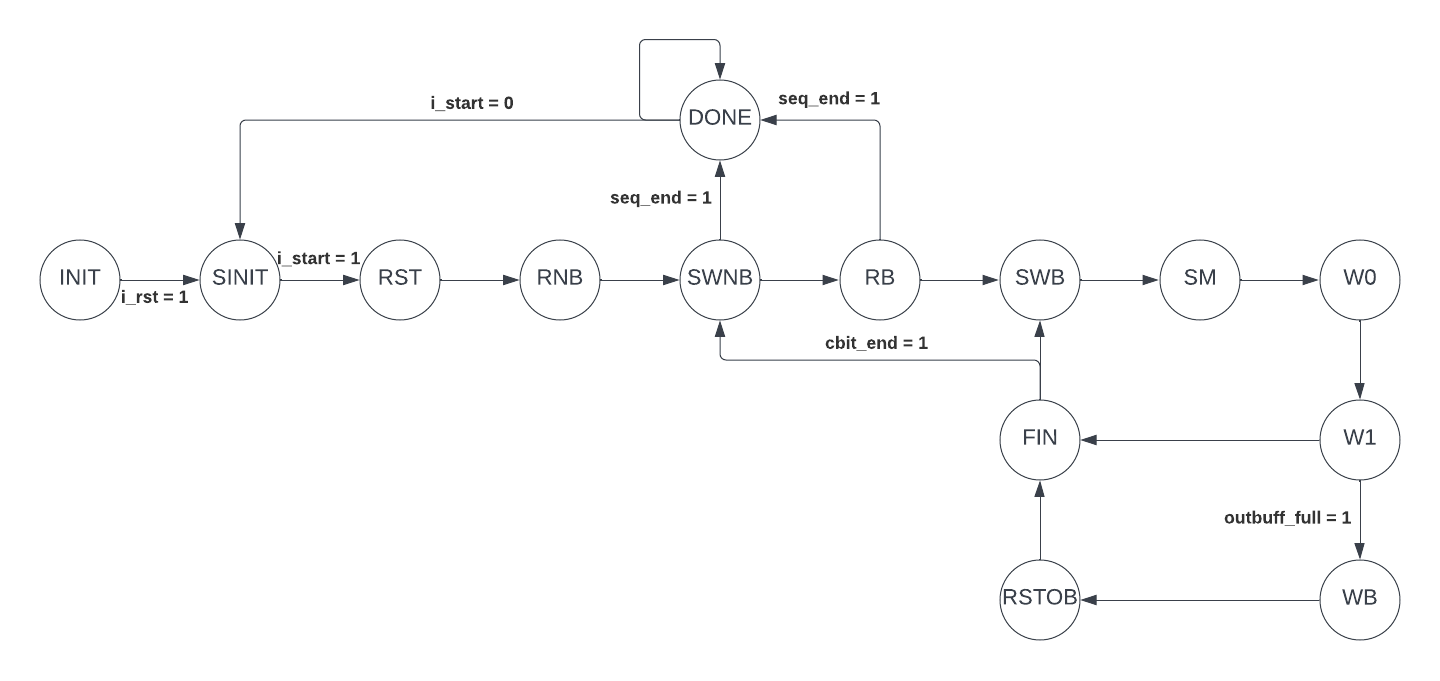
\includegraphics[scale=0.3]{fsm_controllo.png}
    \label{fig:ctrl_fsm}
    \caption{FSM di controllo}
    
\end{figure}

\subsubsection{INIT}
Stato iniziale in cui si trova la macchina prima dell'avvio dell'esecuzione.\\
I segnali di controllo sono tutti disattivati

\subsubsection{SINIT}
Stato in cui si trova la macchina prima dell'avvio di una nuova sequenza\\
I segnali di controllo sono tutti disattivati

\subsubsection{RST}
Reset di tutti i registri interni al datapath per rendere il datapath pronto per
una nuova sequenza.\\
I segnali di controllo attivi sono:
\begin{itemize}
    \item \texttt{sm\_rst} che resetta stato corrente e uscita corrente del convoluzionatore
    \item \texttt{curr\_mux} ad 11 che resetta a la posizione corrente
    \item \texttt{outbuff\_rst} che resetta il buffer di output
    \item \texttt{outbuff\_load} che è necessario per resettare il bufferi di output
\end{itemize}

\subsubsection{RNB}
Lettura del numero di byte dalla RAM ad indirizzo 0.\\
I segnali di controllo attivi sono:
\begin{itemize}
    \item \texttt{nbytes\_load} che attiva il registro che salva il numero di byte da processare
    \item \texttt{curr\_mux} ad 10 che fa avanzare la posizione corrente al prossimo byte
\end{itemize}

\subsubsection{SWNB}
Stato di stallo in attesa della lettura dalla memoria, verifica lo stato corrente ed il termine della sequenza.\\
I segnali di controllo sono tutti disattivati

\subsubsection{RB}
Lettura del byte corrente e memorizzazione nel buffer di input.\\
I segnali di controllo attivi sono:
\begin{itemize}
    \item \texttt{sr\_byte\_load} che attiva la lettura del registro che contiene il byte
\end{itemize}

\subsubsection{SWB}
Stato di stallo in attesa che il byte veng letto con successo.\\
I segnali di controllo attivi sono:
\begin{itemize}
    \item \texttt{sr\_byte\_load} che attiva la lettura del registro che contiene il byte
\end{itemize}

\subsubsection{SM}
Il bit corrente è ora presente all'ingresso del convoluzionatore, che viene abilitato e viene
generato l'output relativo a quel bit.\\
I segnali di controllo attivi sono:
\begin{itemize}
    \item \texttt{sr\_ena} che attiva il registro serializzatore
    \item \texttt{sm\_ena} che attiva il convoluzionatore
\end{itemize}

\subsubsection{W0 e W1}
I bit di output vengono scritti nell'output buffer.\\
Al termine della scrittura si verifica il segnale \texttt{outbuff\_full} per decidere
se è necessario scrivere il buffer di output nella memoria RAM.
I segnali di controllo sono:
\begin{itemize}
    \item \texttt{sm\_w\_sel} rispettivamente a 0 in W0 e 1 in W1 che indica se viene 
                              scritto il bit 0 o il bit 1 del convoluzionatore
    \item \texttt{outbuff\_load} che abilita la scrittura nel buffer di output
\end{itemize}

\subsubsection{WB}
Scrittura del buffer di output in memoria RAM.\\
I segnali di controllo attivi sono:
\begin{itemize}
    \item \texttt{writesel (o\_we)} che attiva il la scrittura in memoria e genera l'indirizzo corretto
\end{itemize}

\subsubsection{RSTOB}
Reset del buffer di output.\\
I segnali di controllo attivi sono:
\begin{itemize}
    \item \texttt{outbuff\_rst} che resetta il buffer di output
    \item \texttt{outbuff\_load} che è necessario per resettare il bufferi di output
\end{itemize}

\subsubsection{FIN}
Il singolo bit è stato processato, viene avanzato il contatore.\\
Si verifica il segnale \texttt{cbit\_end} per decidere se è necessario passare alla lettura del
prossimo byte oppure del prossimo bit.
I segnali di controllo attivi sono:
\begin{itemize}
    \item \texttt{curr\_mux} a 01 che avanza il contatore di una posizione
\end{itemize}

\subsubsection{DONE}
La sequenza è terminata, in attesa di i\_start o i\_rst per iniziare una nuova sequenza.\\
I segnali di controllo attivi sono:
\begin{itemize}
    \item \texttt{o\_done} a 1 che segnala il termine della computazione
\end{itemize}

\pagebreak

\section{Sintesi}

\subsection{Report Utilization}

Il componente è correttamente sintetizzabile, con la versione corrente di Vivado (2021.2) è implementabile su hardware FPGA
xc7a200tfbg484 usando 63 Lookup Tables (LUT) e 53 Flip-Flop.
\\
\\
\noindent In particolare, i 53 flip flop (1 bit a flip flop) sono così ditribuiti:
\begin{itemize}[itemsep=4pt, topsep=4pt]
    \item 4 bit per la macchina a stati di controllo
    \item 2 bit per lo stato corrente del convoluzionatore
    \item 2 bit per l'uscita corrente del convoluzionatore
    \item 8 bit per il buffer di output
    \item 11 bit per la posizione corrente
    \item 8 bit per il byte corrente
    \item 8 bit per il numero di bytes da leggere
    \item 10 bit per segnali di controllo
\end{itemize}

\noindent La sintesi non inferisce latch.

\subsection{Report Timing}

Utilizzando un constraint con clock 15 ns, Vivado (2021.2) riporta
uno Slack (MET) di 11.677 ns ed un Data Path delay di 2.971 ns, quindi c'è margine per
alzare la frequenza del sistema.
\\

\noindent Contenuto del file di constraint:
\begin{minted}{bash}
    create_clock -period 15 -name clock -waveform {0 5} [get_ports i_clk]
\end{minted}

\section{Simulazione e casi di test}

Il componente è stato simulato su una varietà di casi di test, che comprendono anche
gli edge-case più comuni.\\
Viene riportato l'andamento di alcuni segnali in alcune parti della simulazione per una selezione dei casi testati.

\noindent Sono stati effettuati i seguenti casi di test, dei quali per alcuni viene riportata parte della simulazione: %% TODO

\begin{itemize}[itemsep=4pt, topsep=4pt]
    \item test con reset durante l'esecuzione
    \item test con sequenza di lunghezza zero
    \item test con sequenza di lunghezza massima (0xff)
    \item test con cambio della sequenza al termine dell'esecuzione
    \item test con sequenze generate casualmente di lunghezza casuale
\end{itemize}

\pagebreak

\subsubsection{Test con sequenza vuota}

Nel caso la sequenza sia vuota (RAM[0] = 0), dopo la scrittura del numero di bytes nell'apposito registro,
il datapath alzerà immediatamente il segnale \texttt{seq\_end} che porterà la macchina a stati
nello stato di DONE senza mai scrivere nulla in memoria.

\begin{minted}{vhdl}
    seq_end <= '1' when unsigned(curr_pos(10 downto 3)) > nbytes else '0';
\end{minted}

\begin{figure}[h!]
    \centering
    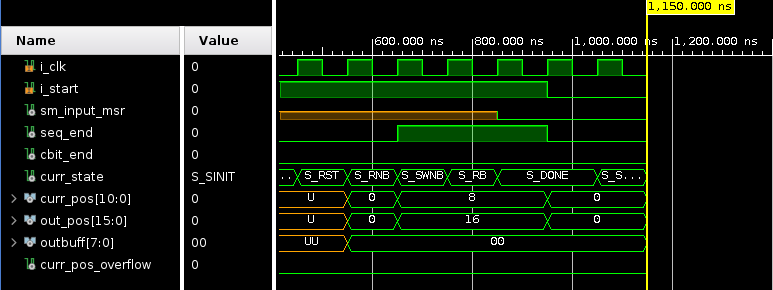
\includegraphics[scale=0.5]{sim_minlen_init.png}
    \label{img:sim_min_init}
    \caption{Simulazione input lunghezza nulla}
\end{figure}

% \pagebreak

\subsubsection{Test con sequenza di lunghezza massima}

Il test con sequenza si lunghezza massima è stato quello con il maggior numero di problemi. \\
Questo perchè dopo aver processato l'ultimo byte il registro \texttt{curr\_pos} va in overflow
nello stato \texttt{FIN} tornando a zero.
\noindent Questo comporta che quando la macchina a stati torna nello stato \texttt{SWNB} con il registro \texttt{curr\_pos} 
che vale zero, minore di \texttt{nbytes}, quindi l'esecuzione riprende dall'inizio.

\noindent Per risolvere il problema è stato quindi introdotto un segnale \texttt{curr\_pos\_overflow} che viene alzato in maniera sequenziale
quando il registro \texttt{curr\_pos} passa da 255 a 0 ed il segnale che pilota il contatore è in posizione "+1" (01)

\noindent Il segnale di fine sequenza è quindi stato modificato per essere attivo anche in caso di
overflow.

\begin{minted}{vhdl}
    seq_end <= '1' when unsigned(curr_pos(10 downto 3)) > nbytes or 
                        curr_pos_overflow = '1' else '0';
\end{minted}

\begin{figure}[h!]
    \centering
    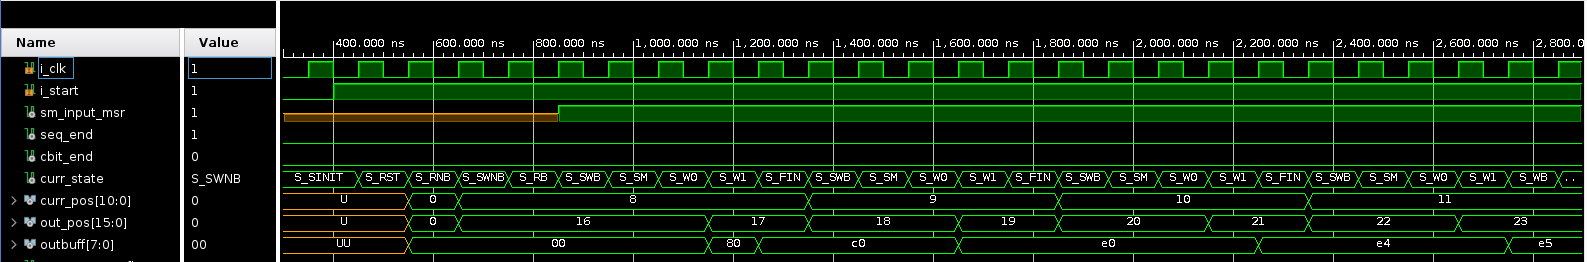
\includegraphics[scale=0.3]{sim_maxlen_init.png}
    \label{img:sim_max_init}
    \caption{Parte iniziale della simulazione con input di lunghezza massima}
\end{figure}

\begin{figure}[h!]
    \centering
    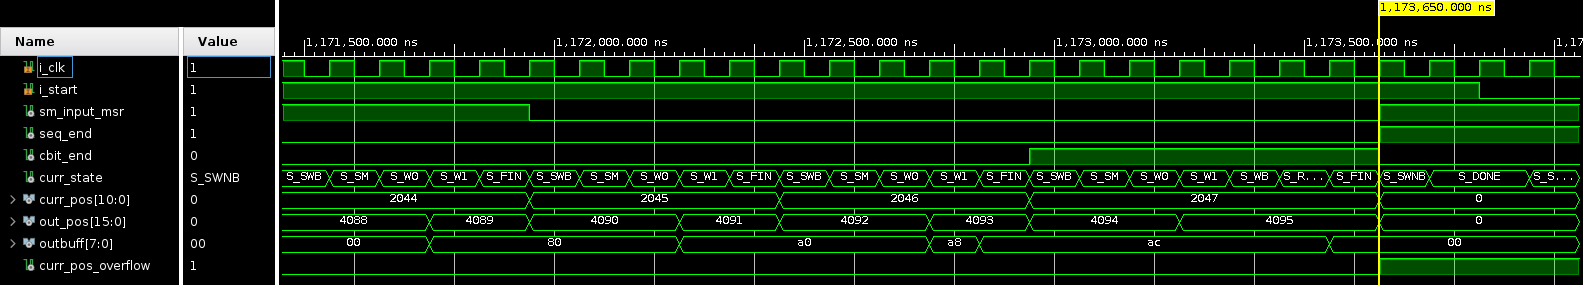
\includegraphics[scale=0.3]{sim_maxlen_end.png}
    \label{img:sim_max_end}
    \caption{Parte finale della simulazione con input di lunghezza massima, si vede curr\_pos andare in overflow e l'alzamento del segnale di overflow}
\end{figure}

%% TODO

\pagebreak

\vspace{10cm}

\subsubsection{Test sequenza con reset}

Quando viene alzato il segnale di reset la FSM di controllo passa sempre nello stato SINIT, ricominciando l'esecuzione.\\
\noindent Quando poi viene alzato il segnale di start la FSM di controllo passa nello stato \texttt{RST}
che provvedere al reset di tutti i componenti interni del datapath e del convoluzionatore.

\begin{minted}{vhdl}
    if i_rst = '1' then
        curr_state <= S_SINIT;
\end{minted}

\subsubsection{Test con sequenze multiple in fila}

Alla fine della sequenza la FSM di controllo alza il segnale \texttt{o\_done}, nel caso in cui \texttt{i\_start} venga abbassato
la macchina si porta nello stato SINIT e si prepara ad accettare una nuova sequenza.

\begin{figure}[h!]
    \centering
    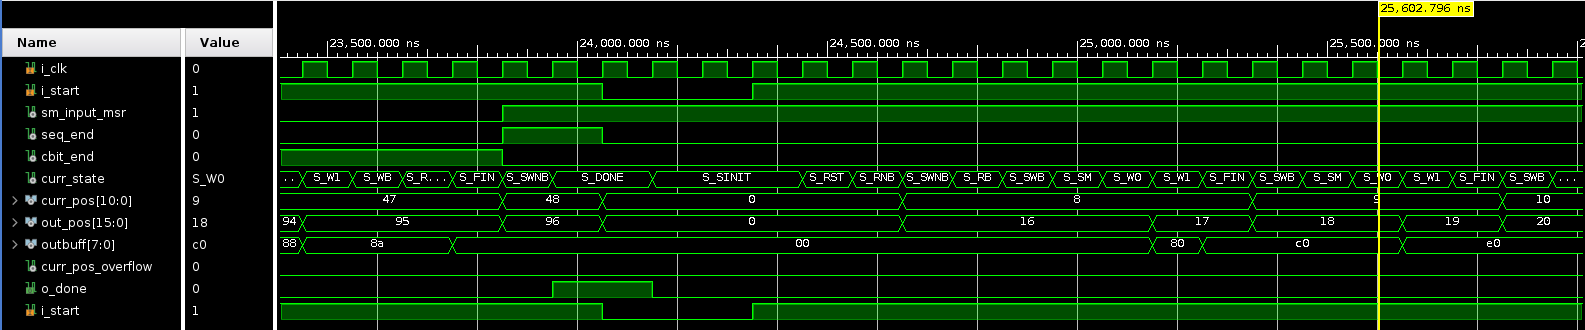
\includegraphics[scale=0.3]{sim_mult_seq.png}
    \label{img:sim_multseq_change}
    \caption{Simulazione fine di una sequenza e inizio della successiva}
\end{figure}

\section{Scelte progettuali}

Si è scelto di scrivere il codice VHDL "a più basso livello" possibile in modo
che la architettura risultante sia il più possibile simile a quella progettata.
Si sarebbe potuto, in alternativa, usare più strutture \texttt{case} ed \texttt{if - elsif} 
al posto di usare MUX e segnali aggiuntivi.


\end{document}